\documentclass[a4paper]{scrreprt}

\usepackage[german]{babel}
\usepackage[utf8]{inputenc}
\usepackage[T1]{fontenc}
\usepackage{ae}
\usepackage[bookmarks,bookmarksnumbered]{hyperref}
\usepackage{graphicx}
\usepackage[toc]{glossaries}
\usepackage{float}
\usepackage{textcomp}
\usepackage{listings}
\usepackage{xcolor}
\lstset{upquote=true}

%===================setting for displaying JSON ==============================
\newcommand\JSONnumbervaluestyle{\color{blue}}
\newcommand\JSONstringvaluestyle{\color{blue}}
% \newcommand\JSONBooleanvaluestyle{\color{blue}}

% switch used as state variable
\newif\ifcolonfoundonthisline

\makeatletter

\lstdefinestyle{json}
{
  showstringspaces    = false,
  keywords            = {false,true},
  alsoletter          = 0123456789.,
  morestring          = [s]{"}{"},
  stringstyle         = \ifcolonfoundonthisline\JSONstringvaluestyle\fi,
  MoreSelectCharTable =%
    \lst@DefSaveDef{`:}\colon@json{\processColon@json},
  basicstyle          = \ttfamily,
  keywordstyle        = \ttfamily\bfseries,
}

% flip the switch if a colon is found in Pmode
\newcommand\processColon@json{%
  \colon@json%
  \ifnum\lst@mode=\lst@Pmode%
    \global\colonfoundonthislinetrue%
  \fi
}

\lst@AddToHook{Output}{%
  \ifcolonfoundonthisline%
    \ifnum\lst@mode=\lst@Pmode%
      \def\lst@thestyle{\JSONnumbervaluestyle}%
    \fi
  \fi
  %override by keyword style if a keyword is detected!
  \lsthk@DetectKeywords%
}

% reset the switch at the end of line
\lst@AddToHook{EOL}%
  {\global\colonfoundonthislinefalse}

\makeatother
%============================================================================


\graphicspath{ {Images/} }
\setcounter{secnumdepth}{5}
\makeglossaries
% \linespread{1.5}

\begin{document}
    \def\code#1{\texttt{#1}}

    \begin{flushright}
        
\includegraphics[scale = 0.7]{kit-logo.jpg}\\[0.5cm]
        % 
\includegraphics[scale = 1]{teco.jpg}
    \end{flushright}
    % 
\includegraphics[scale = 0.5]{kit-logo.jpg} \hspace{4cm} 
\includegraphics[scale = 1]{teco.jpg}
    \vspace*{2cm}

    \begin{center} \large

        Praxis der Softwareentwicklung
        \vspace * {1.5cm}

        \textbf{\huge Mind Rate}

        \vspace*{1cm}


        {\Large Ein interaktives System mit Android-Client f\"ur Studien nach Experience-Sampling-Method (ESM)}

        \vspace*{1cm}

        \textbf{\Large Entwurf}
        \vspace*{2cm}

        Shanshan Du, Yi Ge, Renhan Lou, Ruoheng Ma, Haobin Tan
        \vspace*{1cm}

        02. Dezember 2016
        \vspace*{2.5cm}

        Betreuung: Anja Exler, Dr. Andrea Schankin\\[0.5cm]
        Forschungsgruppe TECO: Technology for Pervasive Computing\\[0.5cm]

        Karlsruher Institut für Technologie
    \end{center}
    \thispagestyle{empty}

    \setlength{\baselineskip}{1.5\baselineskip}{
    \tableofcontents


    \chapter{Allgemeine Struktur}

        Der Entwurf besteht aus zwei Seiten: der Android-App-Seite und der Server-Seite. Sie sind jeweils für die Android-App und das Web-Interface verantwortlich. Zusätzlich soll eine Datenbank auf dem Server laufen, um alle Studien-, Konto- und Probandendaten zu speichern. Diese gehört auch zu der Server-Seite. Die zwei Seiten sollen miteinander durch das HTTP-Protokoll kommunizieren.


        \section{Überblick über die Intekaktion von Android-App und Server}


            \vspace*{1cm}
            \begin{figure}[H]
                % \centering
                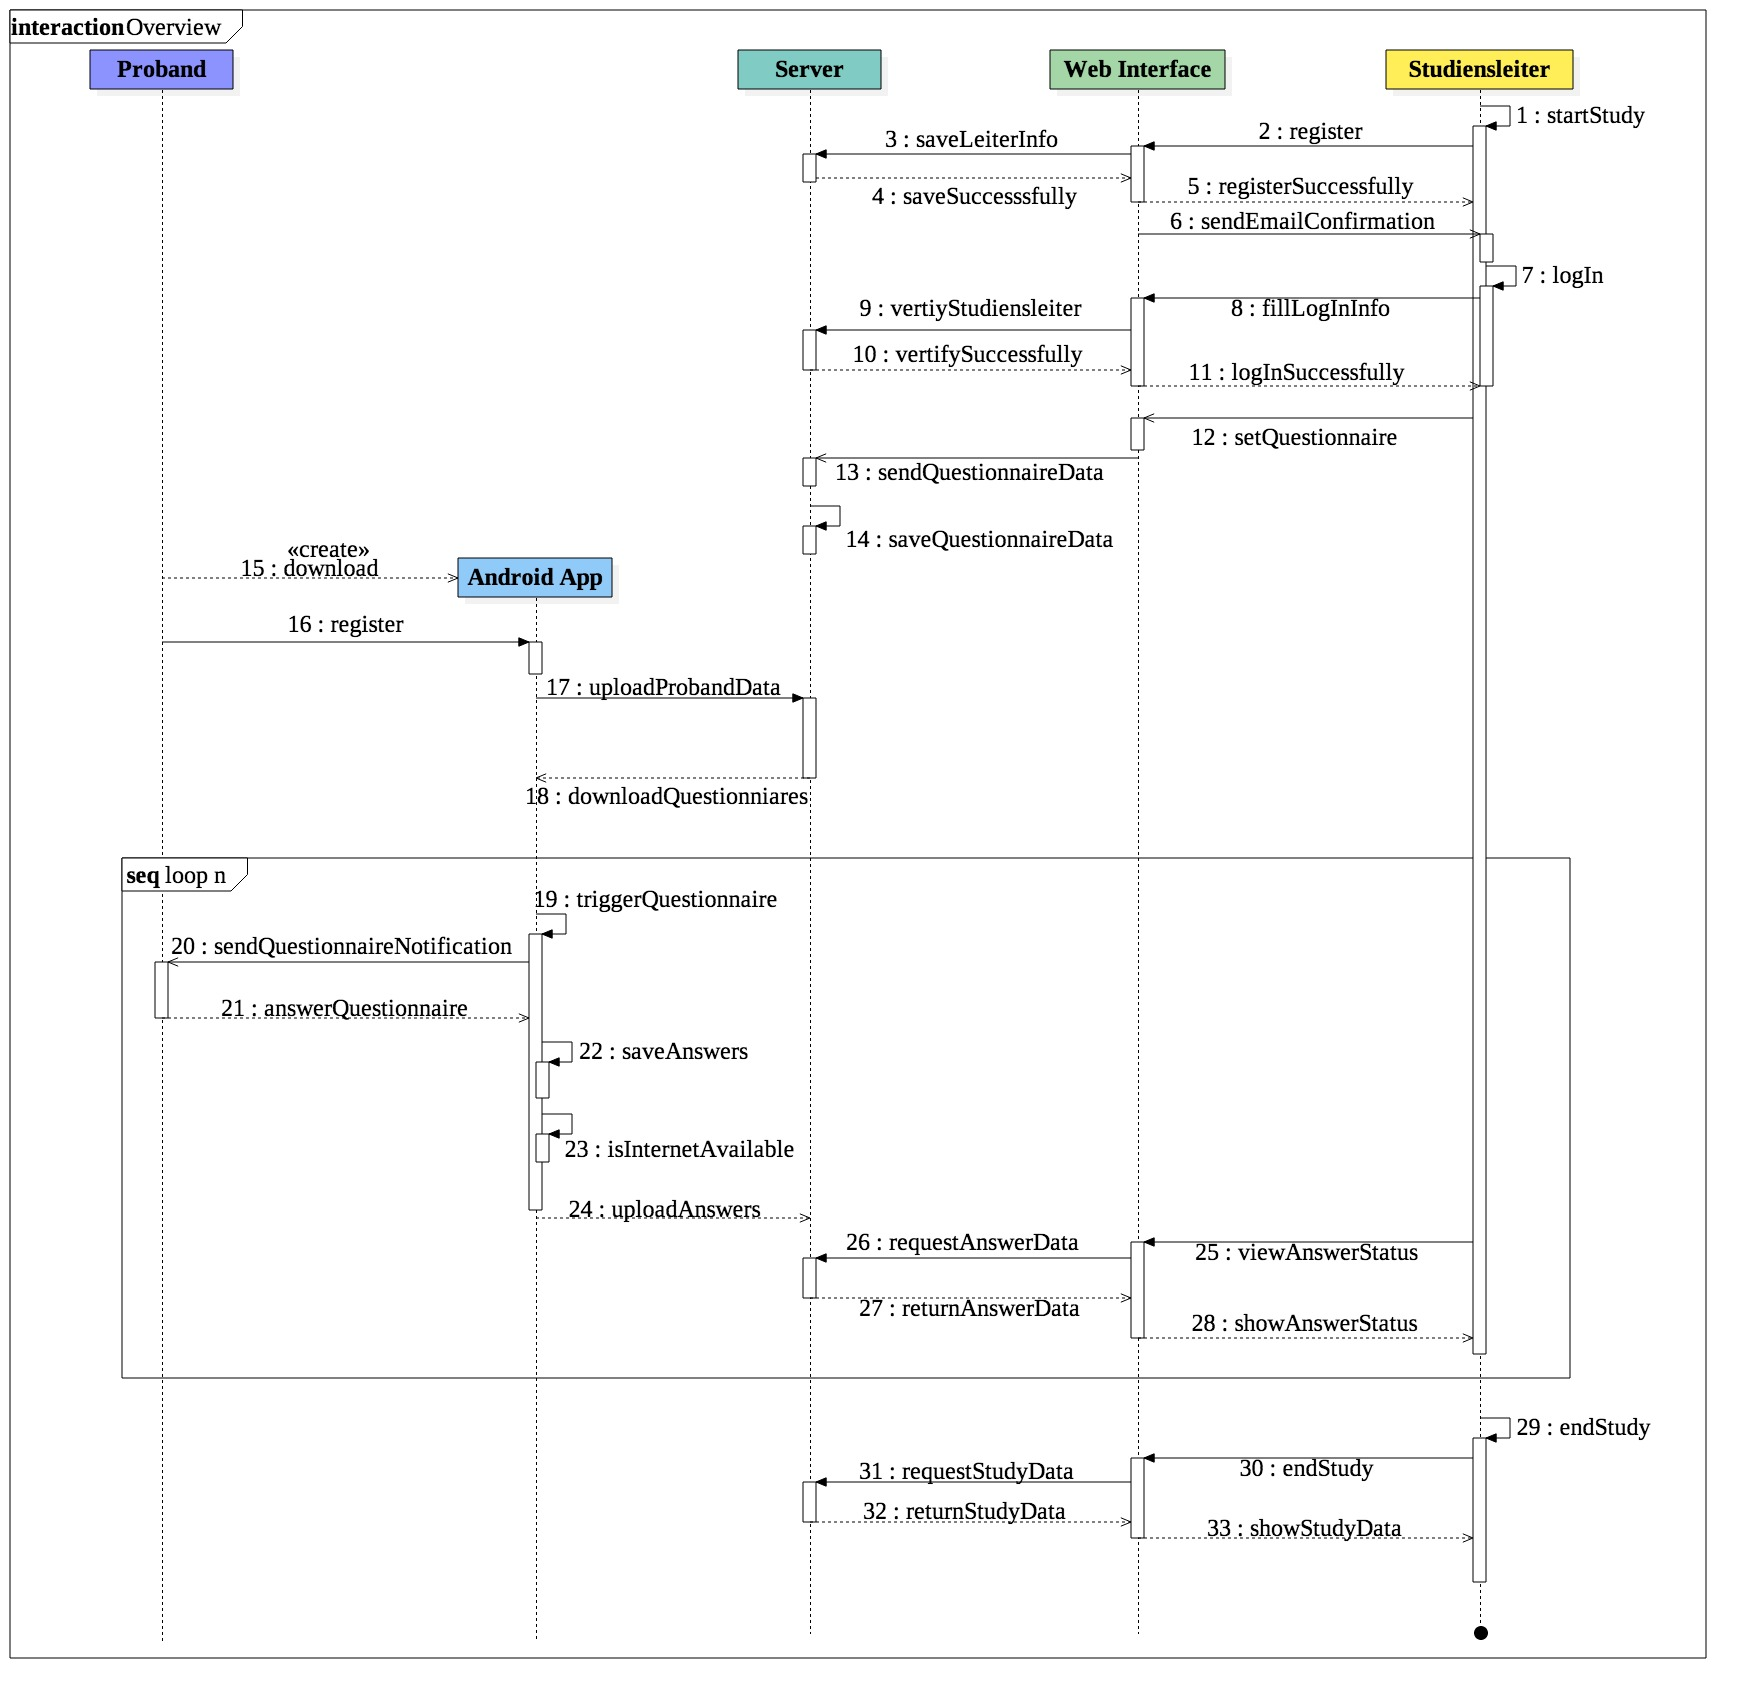
\includegraphics[scale = 0.25]{Overview.jpg}
                \caption{Überblick über die Intekaktion von Android-App und Server}
            \end{figure}



    \chapter{Server-Seite}
        Die Server-Seite nutzt eine von Django-Framework veränderte Variante\footnote{\href{https://docs.djangoproject.com/en/1.10/faq/general/\#django-appears-to-be-a-mvc-framework-but-you-call-the-controller-the-view-and-the-view-the-template-how-come-you-don-t-use-the-standard-names}{https://docs.djangoproject.com/en/1.10/faq/general/\#django-appears-to-be-a-mvc-framework-but-you-call-the-controller-the-view-and-the-view-the-template-how-come-you-don-t-use-the-standard-names}} der Modell-Präsentation-Steuerung-Architektur (MVC) als den Architekturstil. Die benötigte Klassen werden als Modelle entworfen. Der Entwurf von Server-Seite wird auf Python angefertigt.

        \section{Modelle}
            \begin{itemize}
                \item \code{class StudyDirector}
                    \begin{itemize}
                        \item \code{studies = []: Study}
                            \par // a list of all studies that is belonging to this study director
                        \item \code{surname}
                        \item \code{firstName}
                        \item \code{mailAddress}
                            \par // Mail address will also be used as the unique ID of study director.
                    \end{itemize}

                    \item \code{class Study}
                        \begin{itemize}
                            \item \code{probands = []: Proband}
                                \par // a list of all probands that is belonging to this study
                            \item \code{id}
                                \par // unique ID of a study
                            \item \code{name}
                            \item \code{beginningDate: datetime.datetime}
                                \par // using Python datetime module: \code{from datetime import datetime}
                            \item \code{endDate: datetime.datetime}
                            \item \code{director: StudyDirector}
                                \par // the study director of this study
                            \item \code{questionnaires = []: Questionnaire}
                                \par // a list of all questionnaires that is belonging to this study
                        \end{itemize}

                    \item \code{class Proband}
                        \begin{itemize}
                            \item \code{study: Study}
                                \par // the study that this proband attends
                            \item \code{id}
                                \par // the unique ID of a proband
                            \item \code{birthday: datetime.date}
                                \par // using Python datetime module: \code{from datetime import date}
                            \item \code{birthdayRequired: bool}
                            \item \code{occupation}
                            \item \code{occupationRequired: bool}
                            \item \code{gender}
                            \item \code{genderRequired: bool}
                                \par // Only required information will be asked. Otherwise the variables will stay empty.
                        \end{itemize}

                    \item \code{class Questionnairer}
                        \begin{itemize}
                            \item \code{questions = []: AbstractQuestion}
                                \par // a list of all questions
                            \item \code{id}
                                \par // the unique ID of this questionnairer
                            \item \code{name}
                            \item \code{study: Study}
                                \par // the study that this questionnairer is belonging to
                            \item \code{triggerEvent: TriggerEvent}
                                \par // the event that makes the questionnairer to show up
                            \item \code{answeringTime: datetime.timedelta}
                                \par // the time length the probands have to answer the questionnairer after it shows up; using Python datetime module
                            \item \code{answers = []: QuestionnaireAnswer}
                                \par // a list of the questionnairer answers of each proband
                            \item \code{maxShowUpTimesPerDay: int}
                                \par // the maximal times this questionnairer can show up per day
                        \end{itemize}
                        
                    \item \code{class TriggerEvent}
                        \par // The trigger event will only happen when all conditions below are fulfilled at the same time.
                        \begin{itemize}
                            \item \code{minTimeSpace: datetime.timedelta}
                                \par // the minimal time space between two trigger events
                            \item \code{datetime: bool or datetime.datetime}
                                \par // a specific combination of a date and a time; False if this condition is not needed
                            \item \code{time: bool or datetime.time}
                                \par // a time, independent of any particular day; False if this condition is not needed
                            \item \code{triggeredWhenCalendarEventBegins: bool}
                                \par // True if each time a calendar event begins, this condition is fulfilled; False if this condition is not needed
                            \item \code{triggeredWhenCalendarEventEnds: bool}
                                \par // True if each time a calendar event ends, this condition is fulfilled; False if this condition is not needed
                            \item \code{triggeredWhenFacebookNotificationComes: bool}
                                \par // True if each time a Facebook notification comes, this condition is fulfilled; False if this condition is not needed
                            \item \code{triggeredWhenWhatsAppNotificationComes: bool}
                                \par // True if each time a WhatsApp notification comes, this condition is fulfilled; False if this condition is not needed
                            \item \code{linearAcceleration: bool or str}
                                \par // A “>”, “=” or “<” symbol followed by a space and a value; False if this condition is not needed.
                                \par // All the following variables use the same format.
                            \item \code{gravity: bool or str}
                            \item \code{rotation: bool or str}
                                \par // the angle between the device and the ground
                            \item \code{airTemperature: bool or str}
                            \item \code{airPressure: bool or str}
                            \item \code{light: bool or str}
                                \par // ambient light level in SI lux units
                            \item \code{relativeHumidity: bool or str}
                            \item \code{orientation: bool or str}
                                \par // Angle between the magnetic north direction and the y-axis of the device, around the z-axis (0 to 359). 0 = North, 90 = East, 180 = South, 270 = West
                            \item \code{magneticField: bool or str}
                            \item \code{proximity: bool or str}
                                \par // proximity sensor distance measured in centimeters
                        \end{itemize}

                    \item \code{class QuestionnaireAnswer}
                        \begin{itemize}
                            \item \code{submitter: Proband}
                            \item \code{submitTime: datetime.datetime}
                            \item \code{fulfilledTriggerConditions: dict}
                                \par // The fulfilled condition values when the trigger event happens; keys of the dictionary are the condition names, values are the condition values when triggered.
                            \item \code{questionAnswers = []: AbstractQuestionAnswer}
                                \par // all question answers in a questionnairer
                        \end{itemize}

                    \item \code{class AbstractQuestion(ABC)}
                        \par // an abstract question class that extends the Python Abstract Base Classes (ABC): \code{from abc import ABC, abstractmethod}
                        \begin{itemize}
                            \item \code{id}
                            \item \code{questionnaire: Questionnaire}
                            \item \code{showByDefault: bool = True}
                                \par // False if the question is hidden by default, and will only be showed if it is triggered as a follow up question; the proband will only see it if he chooses the trigger option of the previous question.
                            \item \code{content: str}
                            \item \code{@abstractmethod} \\
                                       \code{def getContent(self): dict}
                                \par // a unique method of getting the content of a question
                                \par // The answer will be a dictionary, in which the value of the “type” key will be the string name of the question type like \verb|"TextQuestion"| or \verb|"ChoiceQuestion"|, and the other elements will be different for each question types.
                        \end{itemize}

                    \item \code{class TextQuestion(AbstractQuestion)}
                        \begin{itemize}
                            \item \code{id}
                            \item \code{questionnaire: Questionnaire}
                            \item \code{showByDefault: bool = True}
                            \item \code{content: str}
                            \item \code{def getContent(self): dict}
                                \par // The value of the “content” key is the \code{content} attribute.
                        \end{itemize}

                    \item \code{class ChoiceQuestion(AbstractQuestion)}
                        \par // Both single choice question and multiple choice question are belonging to this class.
                        \begin{itemize}
                            \item \code{id}
                            \item \code{questionnaire: Questionnaire}
                            \item \code{showByDefault: bool = True}
                            \item \code{content: str}
                            \item \code{options = []}
                            \item \code{followUpQuestion: bool or AbstractQuestion}
                                \par // False if there is no follow up question.
                            \item \code{followUpQuestionTriggerOptions = []}
                                \par // The follow up question will only show up, if one or more of the specific options of this question is chosen.
                            \item \code{def getContent(self): dict}
                                \par // The value of the “content” key is the \code{content} attribute; the value of the “options” key is the \code{options} list.
                        \end{itemize}

                    \item \code{class SteplessScaleQuestion(AbstractQuestion)}
                        \begin{itemize}
                            \item \code{id}
                            \item \code{questionnaire: Questionnaire}
                            \item \code{showByDefault: bool = True}
                            \item \code{content: str}
                            \item \code{scaleMin: int}
                            \item \code{scaleMax: int}
                            \item \code{followUpQuestion: bool or AbstractQuestion}
                                \par // False if there is no follow up question.
                            \item \code{followUpQuestionTriggerMin: int}
                            \item \code{followUpQuestionTriggerMax: int}
                                \par // The follow up question will only show up, if the answer falls within the trigger interval.
                            \item \code{def getContent(self): dict}
                               \par // The dictionary has both “scaleMin” and “scaleMax” keys. The value of the “content” key is the \code{content} attribute.
                        \end{itemize}
                        
                    \item \code{class ScaleQuestionWithSteps(AbstractQuestion)}
                        \begin{itemize}
                            \item \code{id}
                            \item \code{questionnaire: Questionnaire}
                            \item \code{showByDefault: bool = True}
                            \item \code{content: str}
                            \item \code{hasThreeSteps: bool}
                            \item \code{hasFiveSteps: bool}
                            \item \code{hasSevenSteps: bool}
                                \par // Only one of the above boolean values can be true; the question has either 3, 5 or 7 steps.
                            \item \code{stepNames = []}
                                \par // Each step can have a name; \code{len(steps)} must be 3, 5 or 7 according to the step amount.
                            \item \code{followUpQuestion: bool or AbstractQuestion}
                                \par // False if there is no follow up question.
                            \item \code{followUpQuestionTriggerStep: []}
                                \par // The follow up question will only show up, if one of the specific steps is chosen.
                            \item \code{def getContent(self): dict}
                               \par // The value of the “stepNumber” key is either 3, 5 or 7. The value of the “stepNames” key is the \code{stepNames} list. The value of the “content” key is the \code{content} attribute.
                        \end{itemize}

                    \item \code{class AbstractQuestionAnswer(ABC)}
                        \begin{itemize}
                            \item \code{content}
                        \end{itemize}

                   \item \code{class TextQuestionAnswer(AbstractQuestionAnswer)}
                       \begin{itemize}
                           \item \code{content: string}
                       \end{itemize}

                    \item \code{class SingleChoiceQuestionAnswer(AbstractQuestionAnswer)}
                        \begin{itemize}
                            \item \code{content: int}
                                \par // the index of the chosen option beginning from 0
                        \end{itemize}
                        
                   \item \code{class MultiChoiceQuestionAnswer(AbstractQuestionAnswer)}
                       \begin{itemize}
                           \item \code{content = []: int}
                               \par // a list of the indices of the chosen options beginning from 0
                       \end{itemize}
                       
                    \item \code{class SteplessScaleQuestionAnswer(AbstractQuestionAnswer)}
                        \begin{itemize}
                            \item \code{content: double}
                                \par // the chosen value that is greater than the “scaleMin” and smaller than the “scaleMax” values of the question
                        \end{itemize}
                        
                    \item \code{class ScaleQuestionWithStepsAnswer(AbstractQuestionAnswer)}
                        \begin{itemize}
                            \item \code{content: int}
                                \par // the index of the chosen step beginning from 0
                        \end{itemize}

            \end{itemize}

        \newpage
        \section{Entity-Relationship-Modell der Datenbank}
            \begin{figure}[ht]
                \centering
                %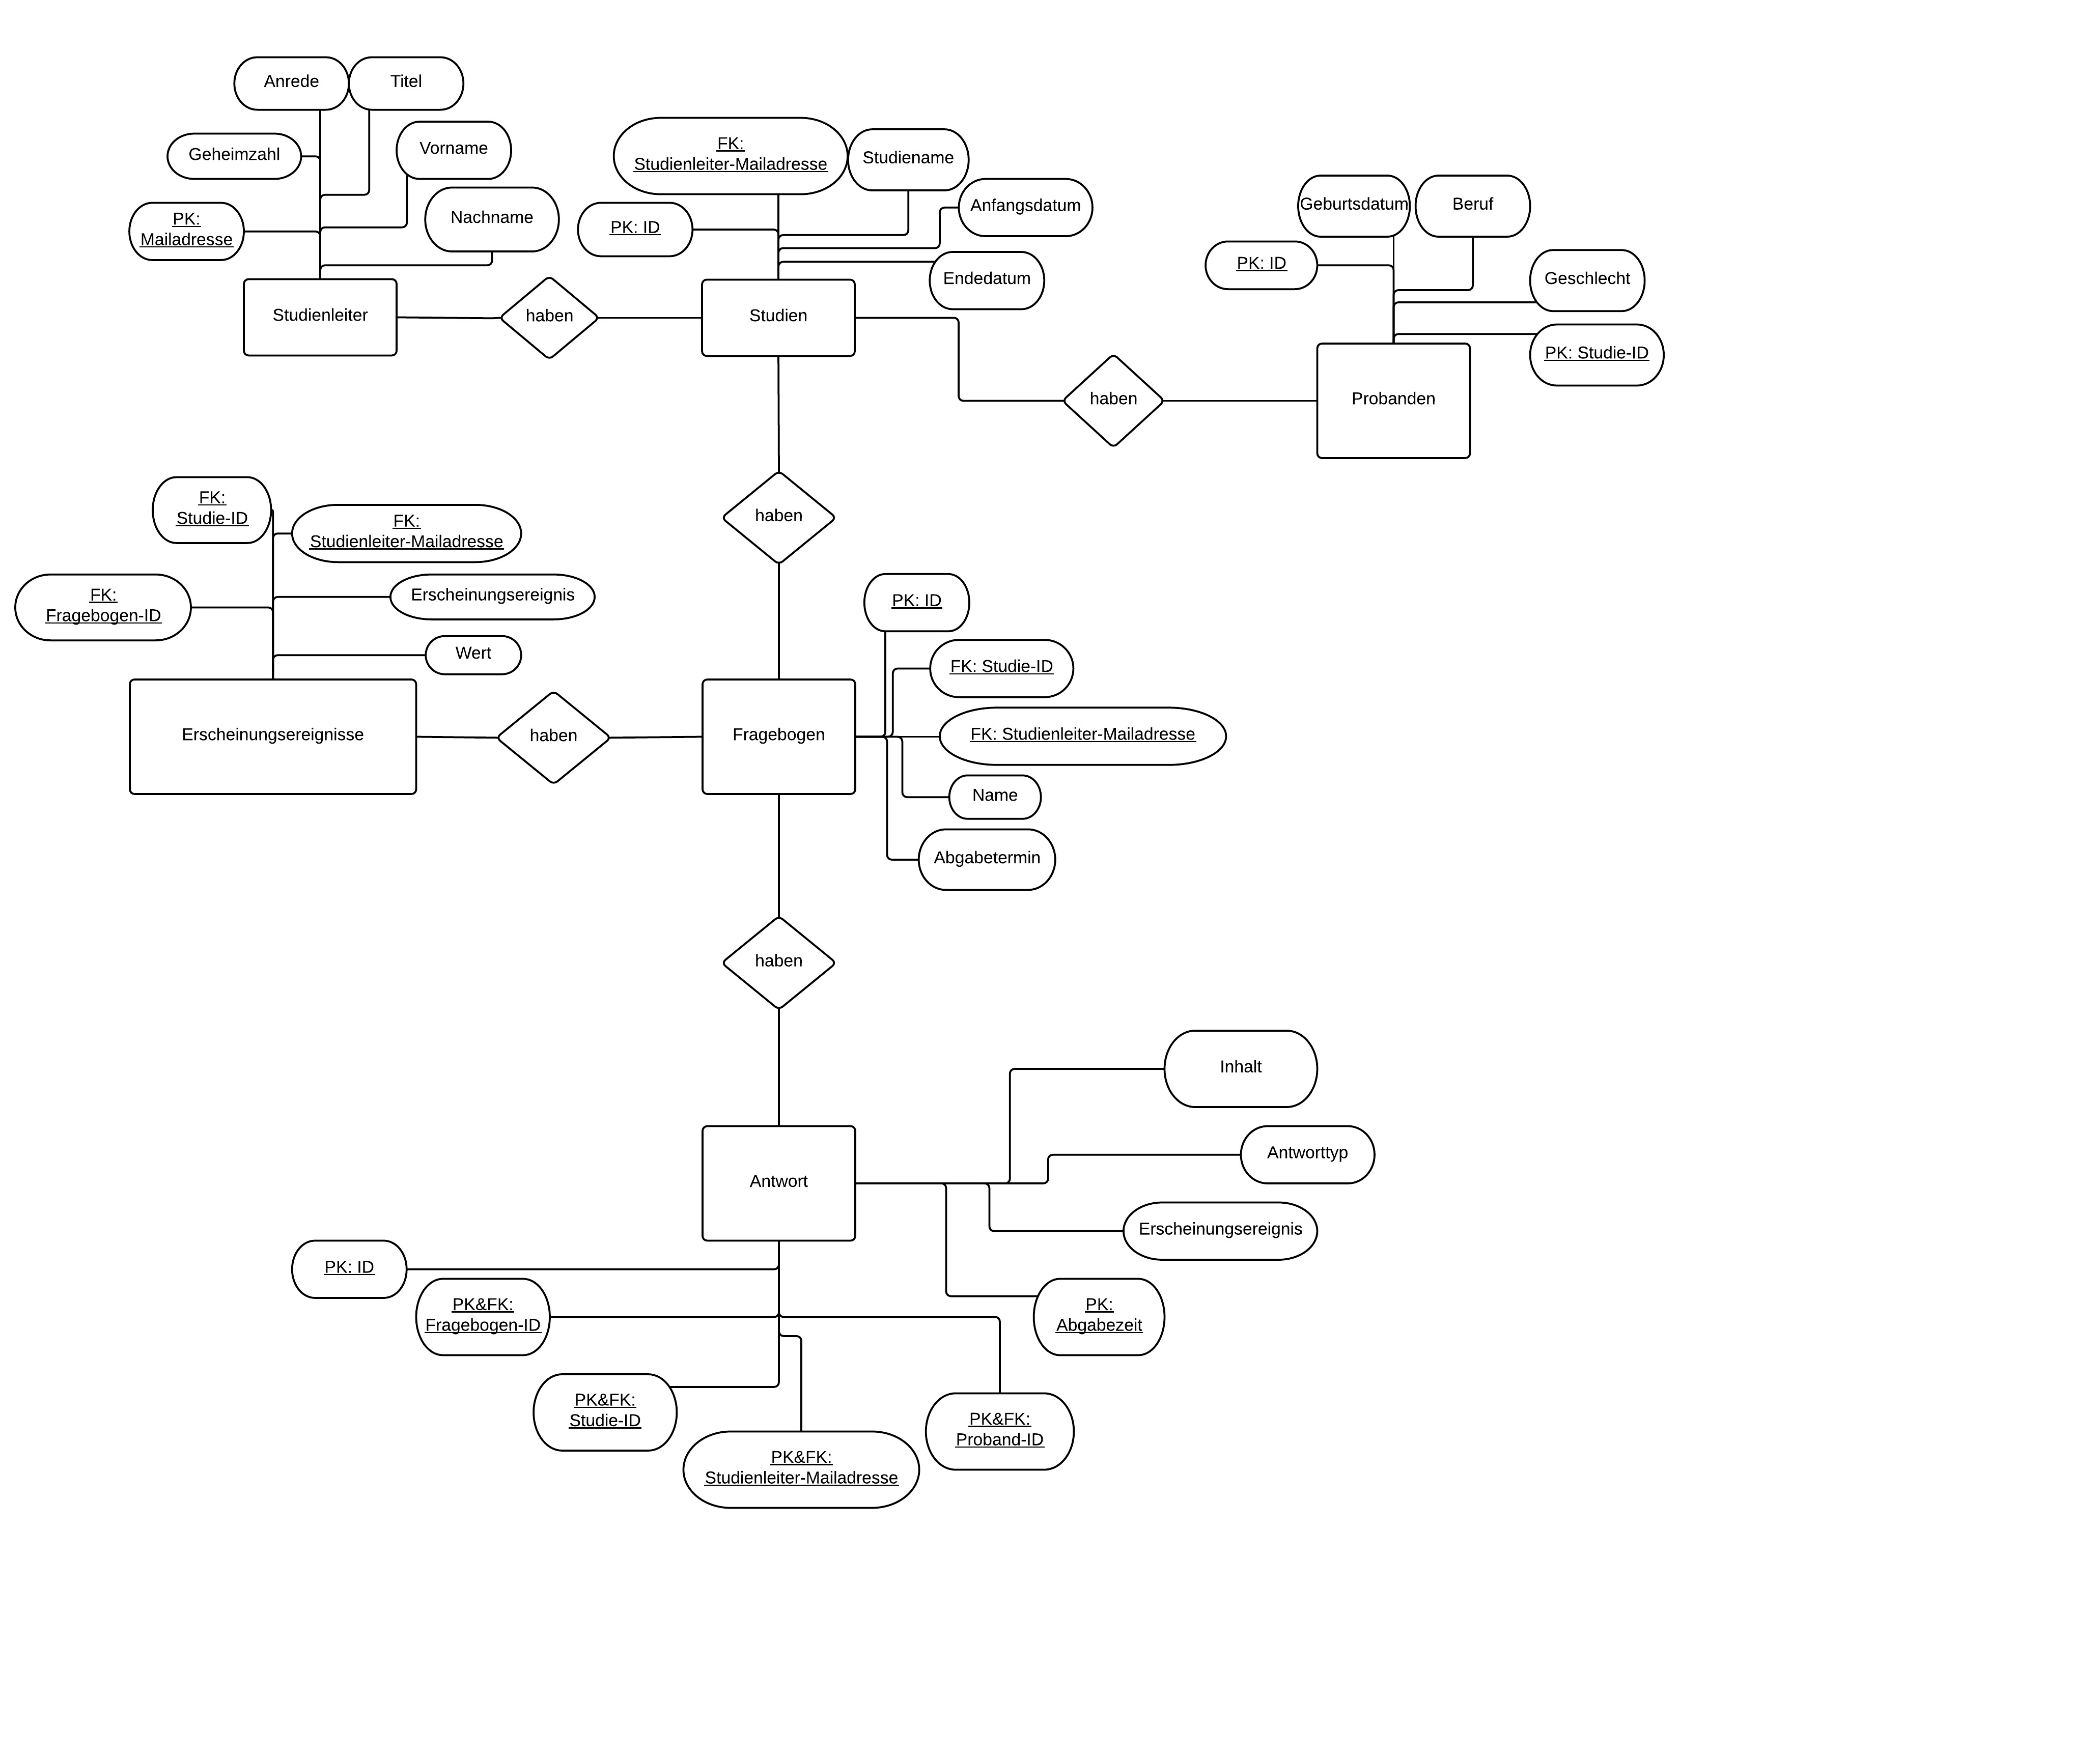
\includegraphics[scale = 0.13]{PSE_Datenbank_ERM.jpeg}
                \caption{Entity-Relationship-Modell der Datenbank}
            \end{figure}


    \newpage
    % \setlength{\baselineskip}{1.5\baselineskip}{
    \chapter{Android-App}

        Das Entwurfsmuster Model-View-Controller (MVC, englisch für Modell-Präsentation-Steuerung) wird hier angewandet, um einen fleixbler Programmentwurf zu ermöglichen.


        \vspace*{0.5cm}
        \section{Überblick über Pakete}

            Das folgende Diagramm dient sich als einen Überblick über unsere Android App. Modell, Präsentation und Steuerung werden mit drei verschiedenen Farbe dargestellt: blau für Modell, grün für Präsentation und gelb für Steuerung.

            \noindent Um die Beziehungen zwischen Klassen und das System ganzheitlich aufzufassen, enthält folgendes Diagramm keine Attribute und Methoden. Jede Pakete sowie Klasse mit Attribute und (offene) Methoden werden dann ausführlich beschrieben.



            \newpage
            \vspace*{1cm}
            \begin{figure}[H]
                \centering
                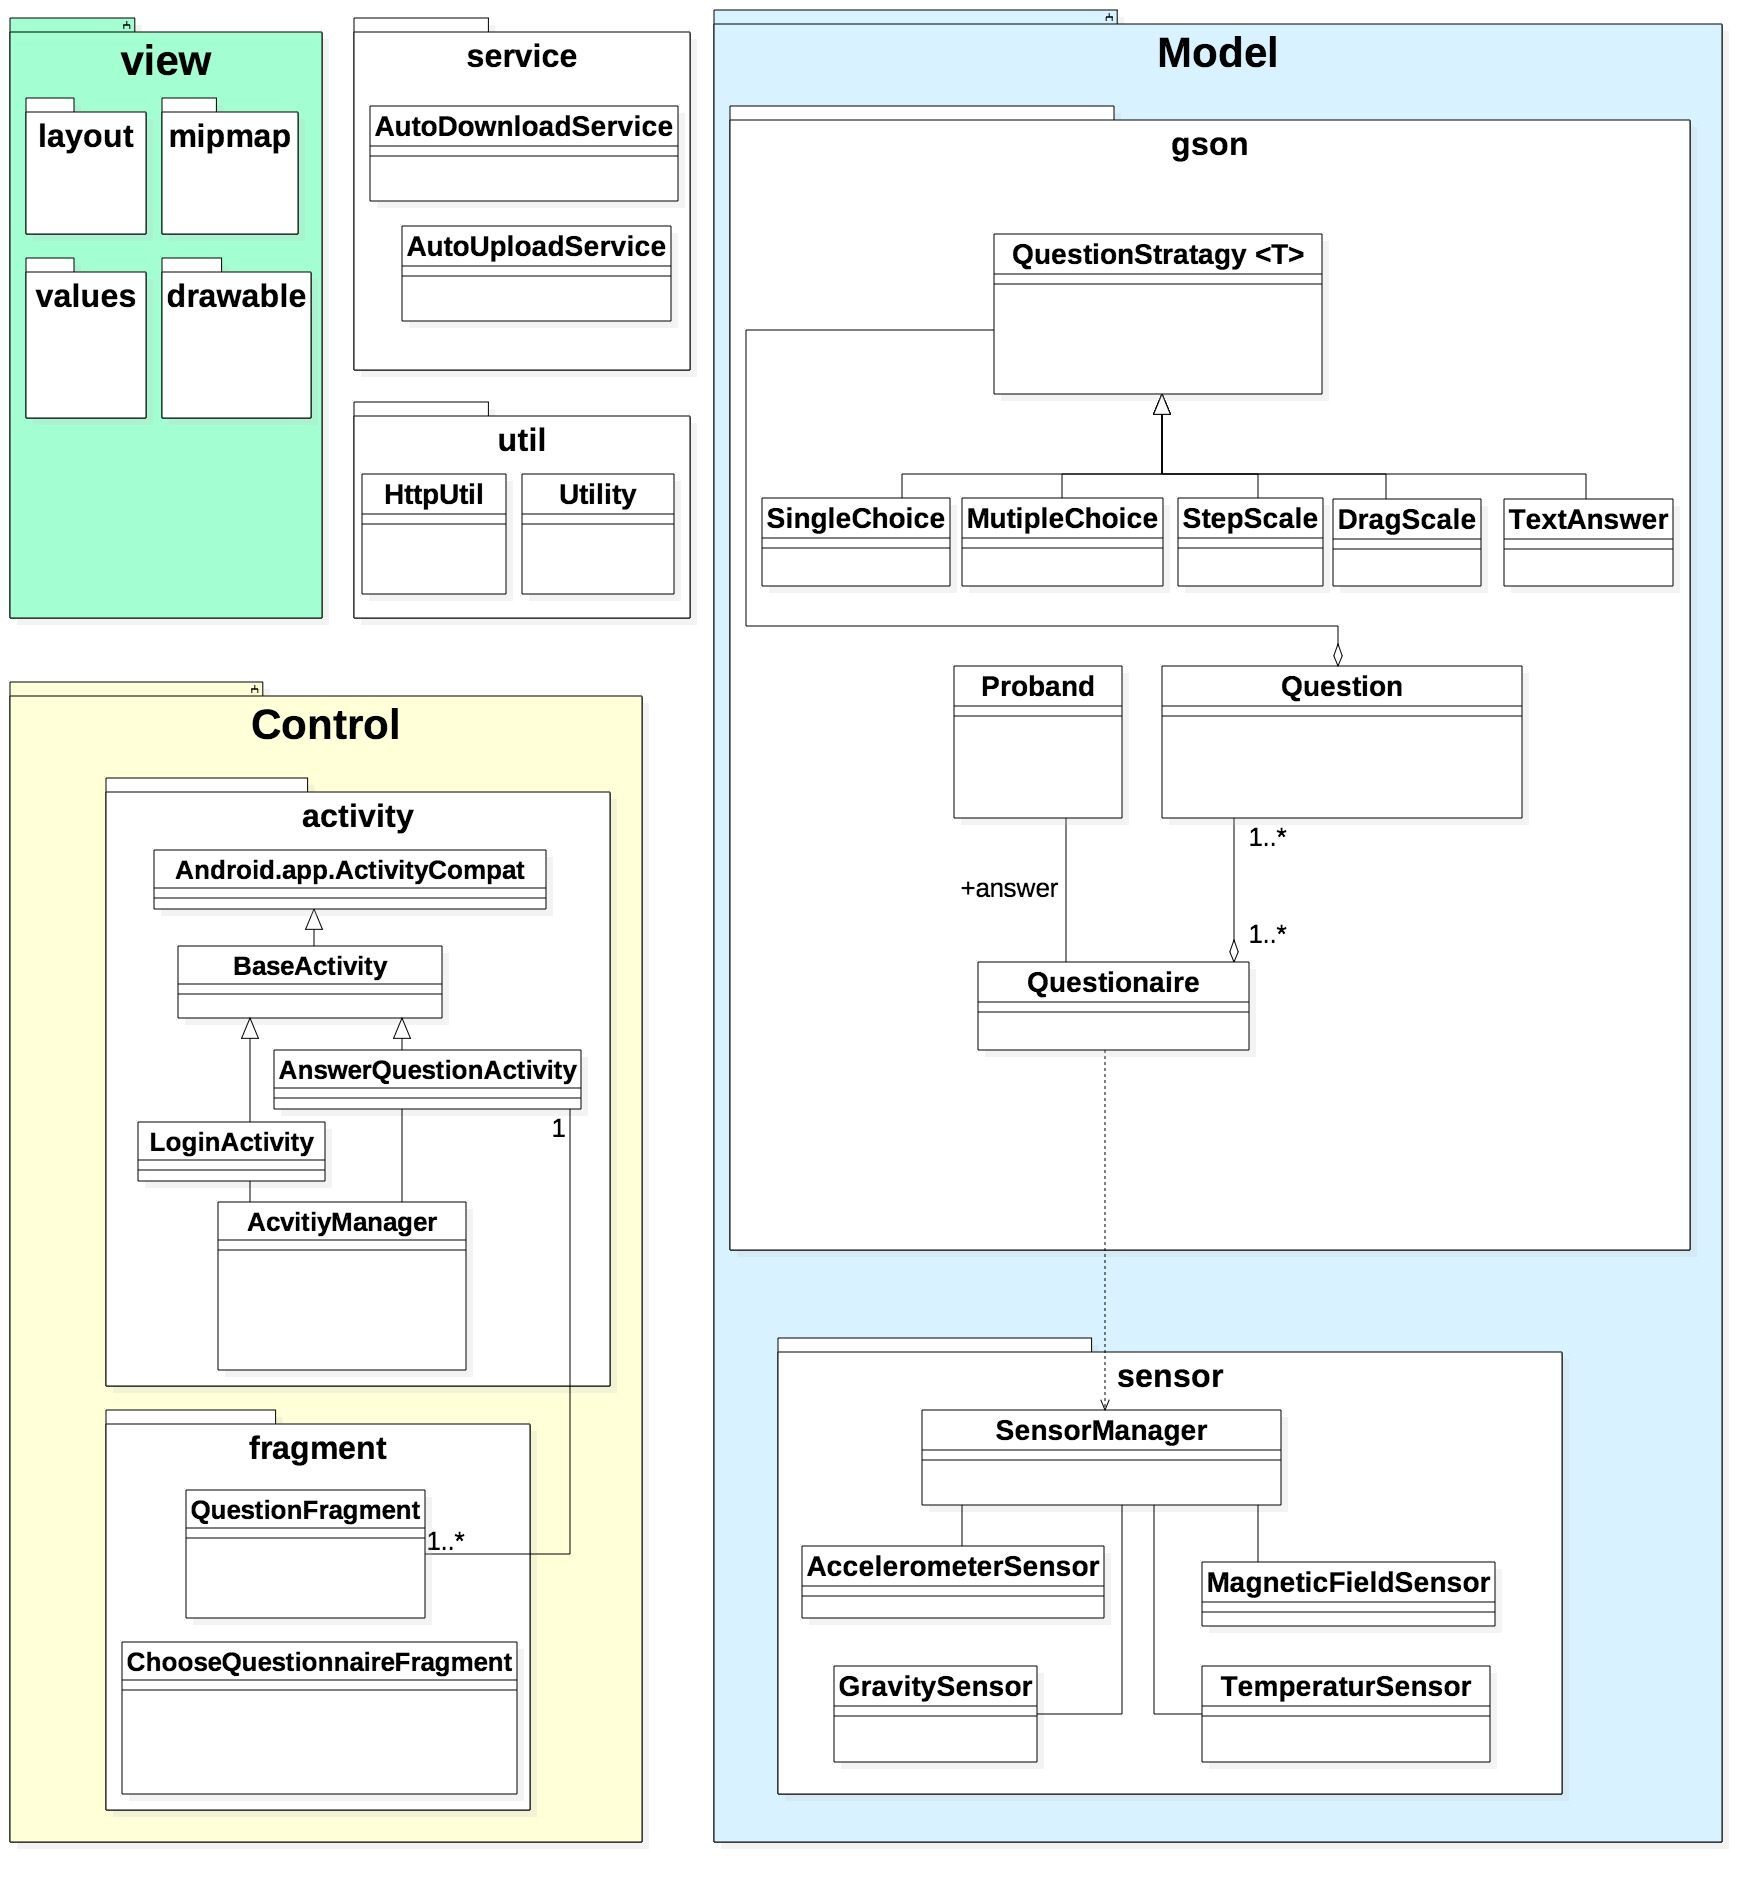
\includegraphics[scale = 0.25]{packageDiagram.jpg}
                \caption{Überblick über alle Packte und Klasse (ohne Attribute und Methoden)}
            \end{figure}




        %TODO: Ausführliche Beschreibung für jedes package und klasse davon


        \section{Model}

            Der Teil Model besteht aus zwei Pakete:

            \begin{itemize}
                \item package \code{gson}
                    \begin{itemize}
                        \item \code{abstract class QuestionStrategy}
                        \item \code{class SingleChoice}
                        \item \code{class MutipleChoice}
                        \item \code{class StepScale}
                        \item \code{class DragScale}
                        \item \code{class TextAnswer}
                        \item \code{class Proband}
                        \item \code{class Questionnaire}
                        \item \code{class Question}
                    \end{itemize}
                \item package \code{sensor}
                    \begin{itemize}
                        \item \code{SensorManager}
                        \item \code{AccelerometerSensor}
                        \item \code{MagneticFeldSensor}
                        \item \code{GravitySensor}
                        \item \code{TemperatureSensor}
                    \end{itemize}
            \end{itemize}

            \begin{figure}[H]
                \centering
                % 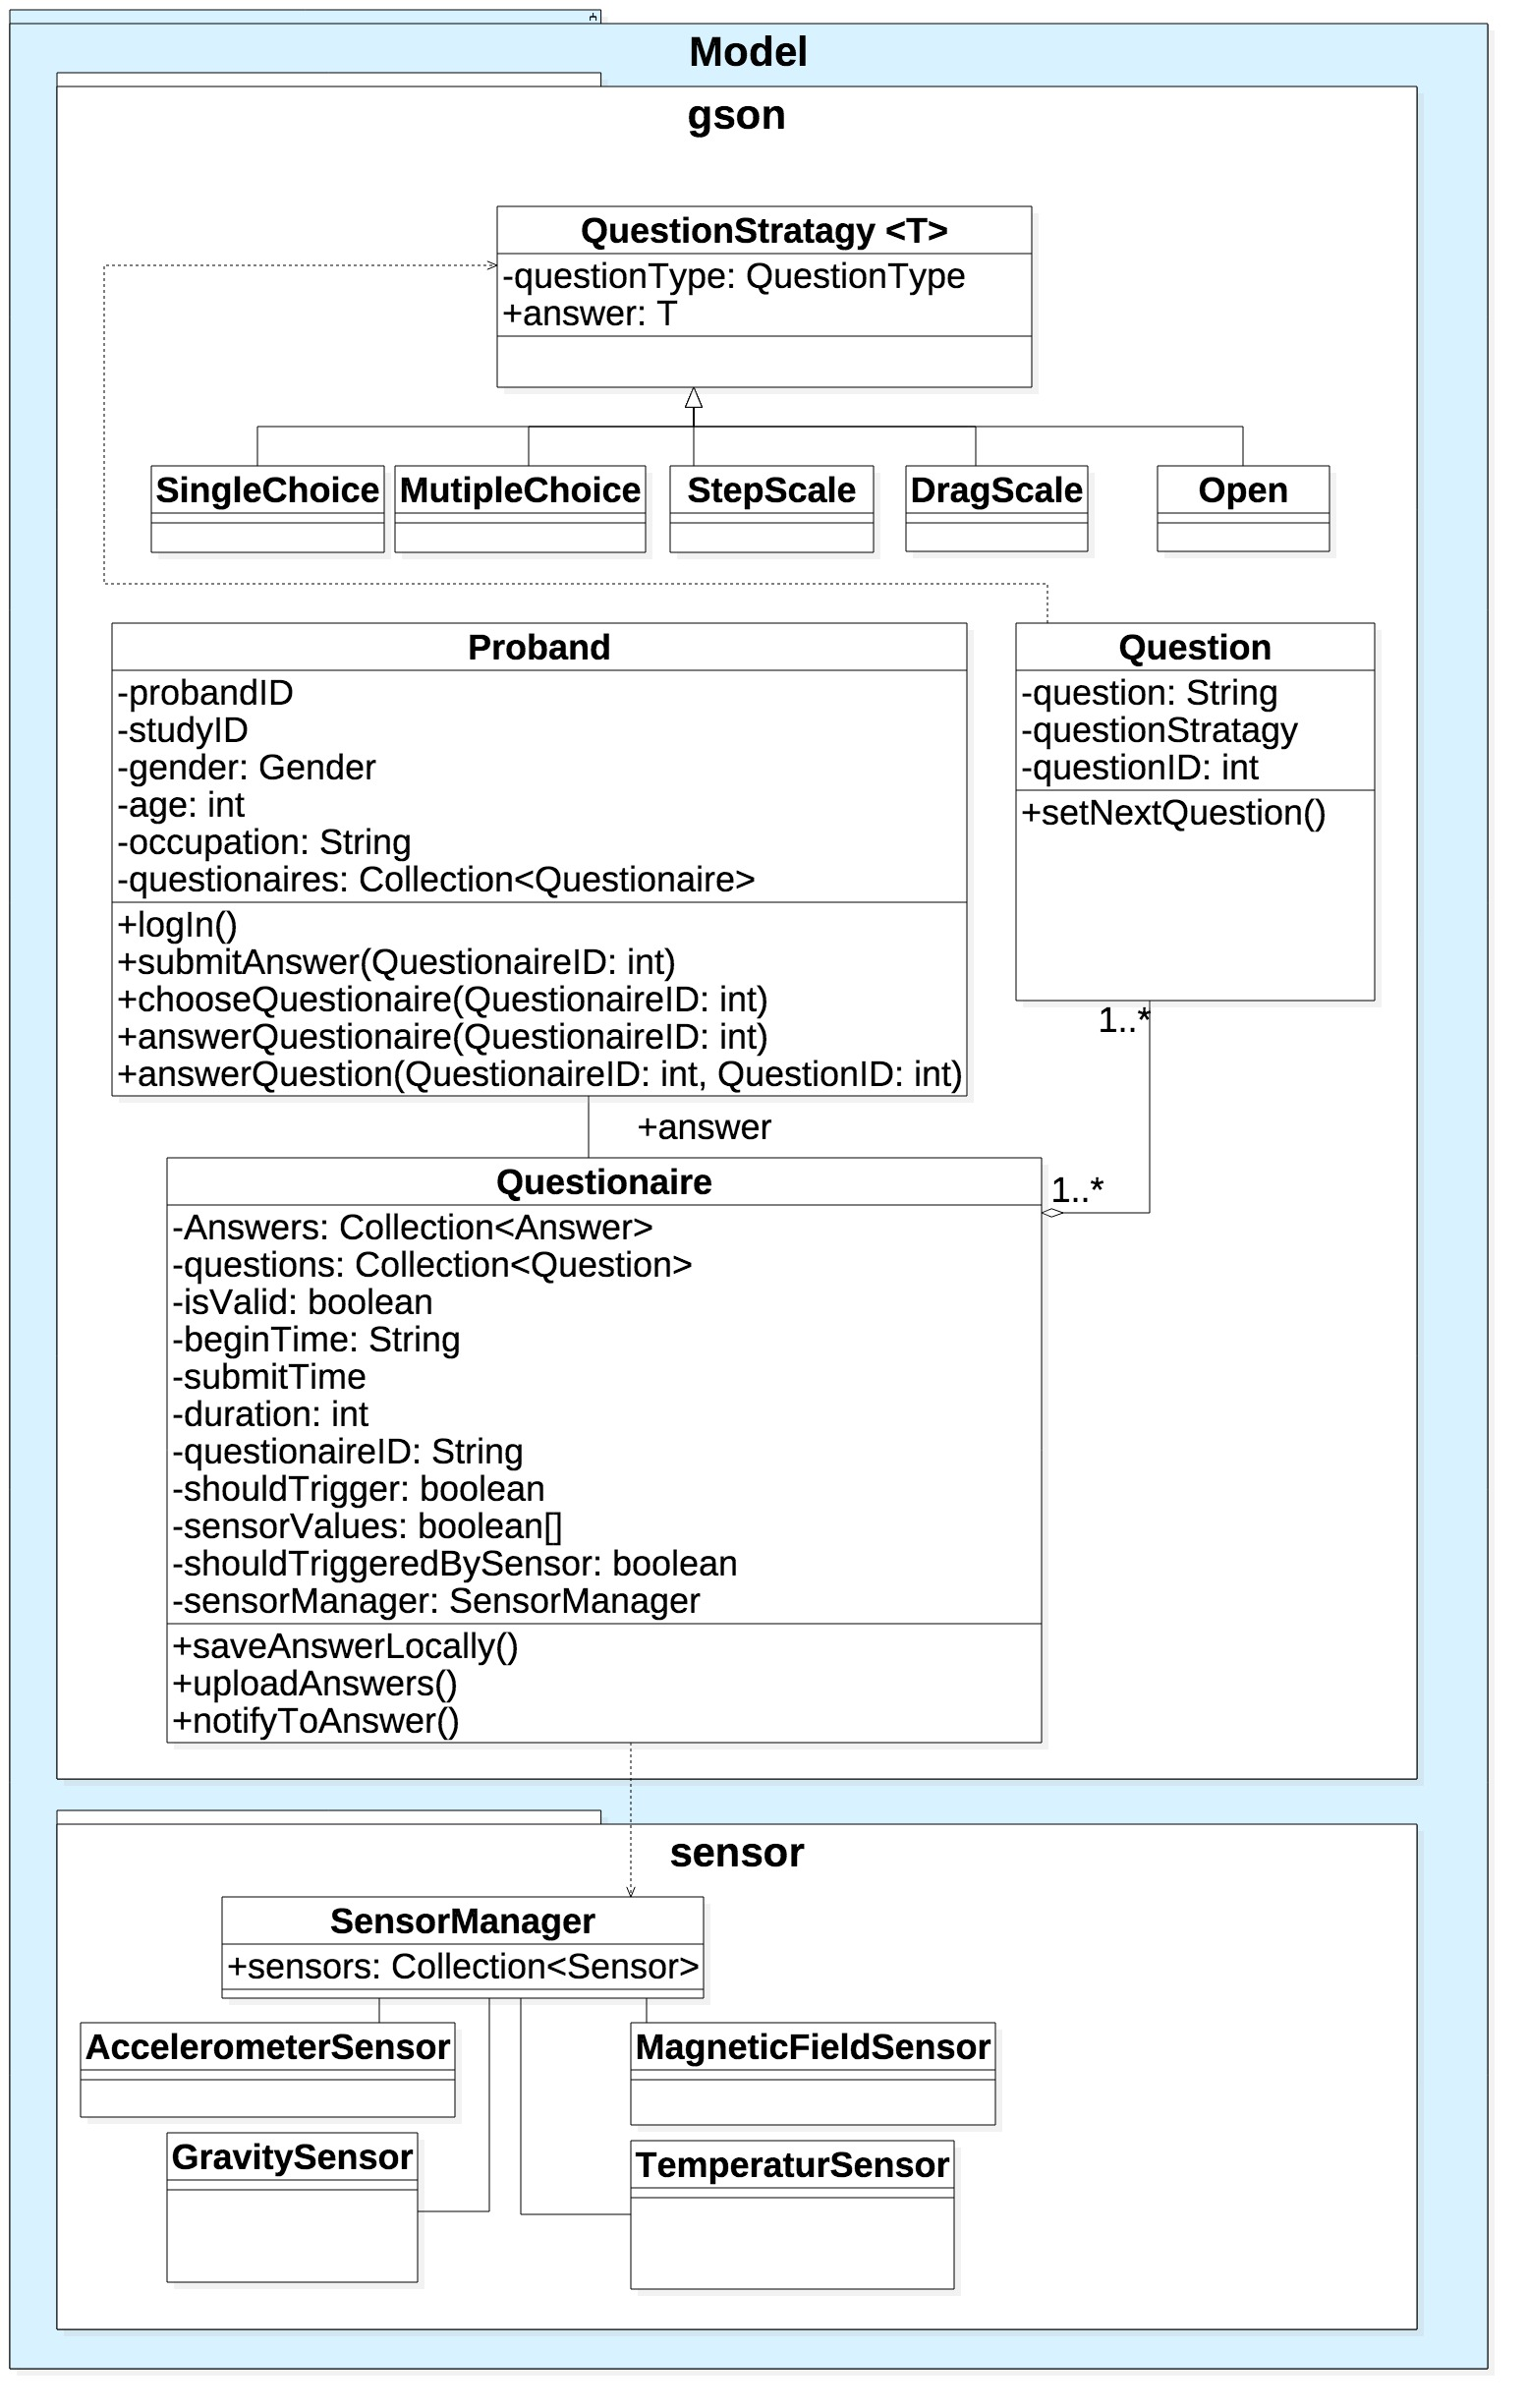
\includegraphics[scale = 0.25]{Model.jpg}
                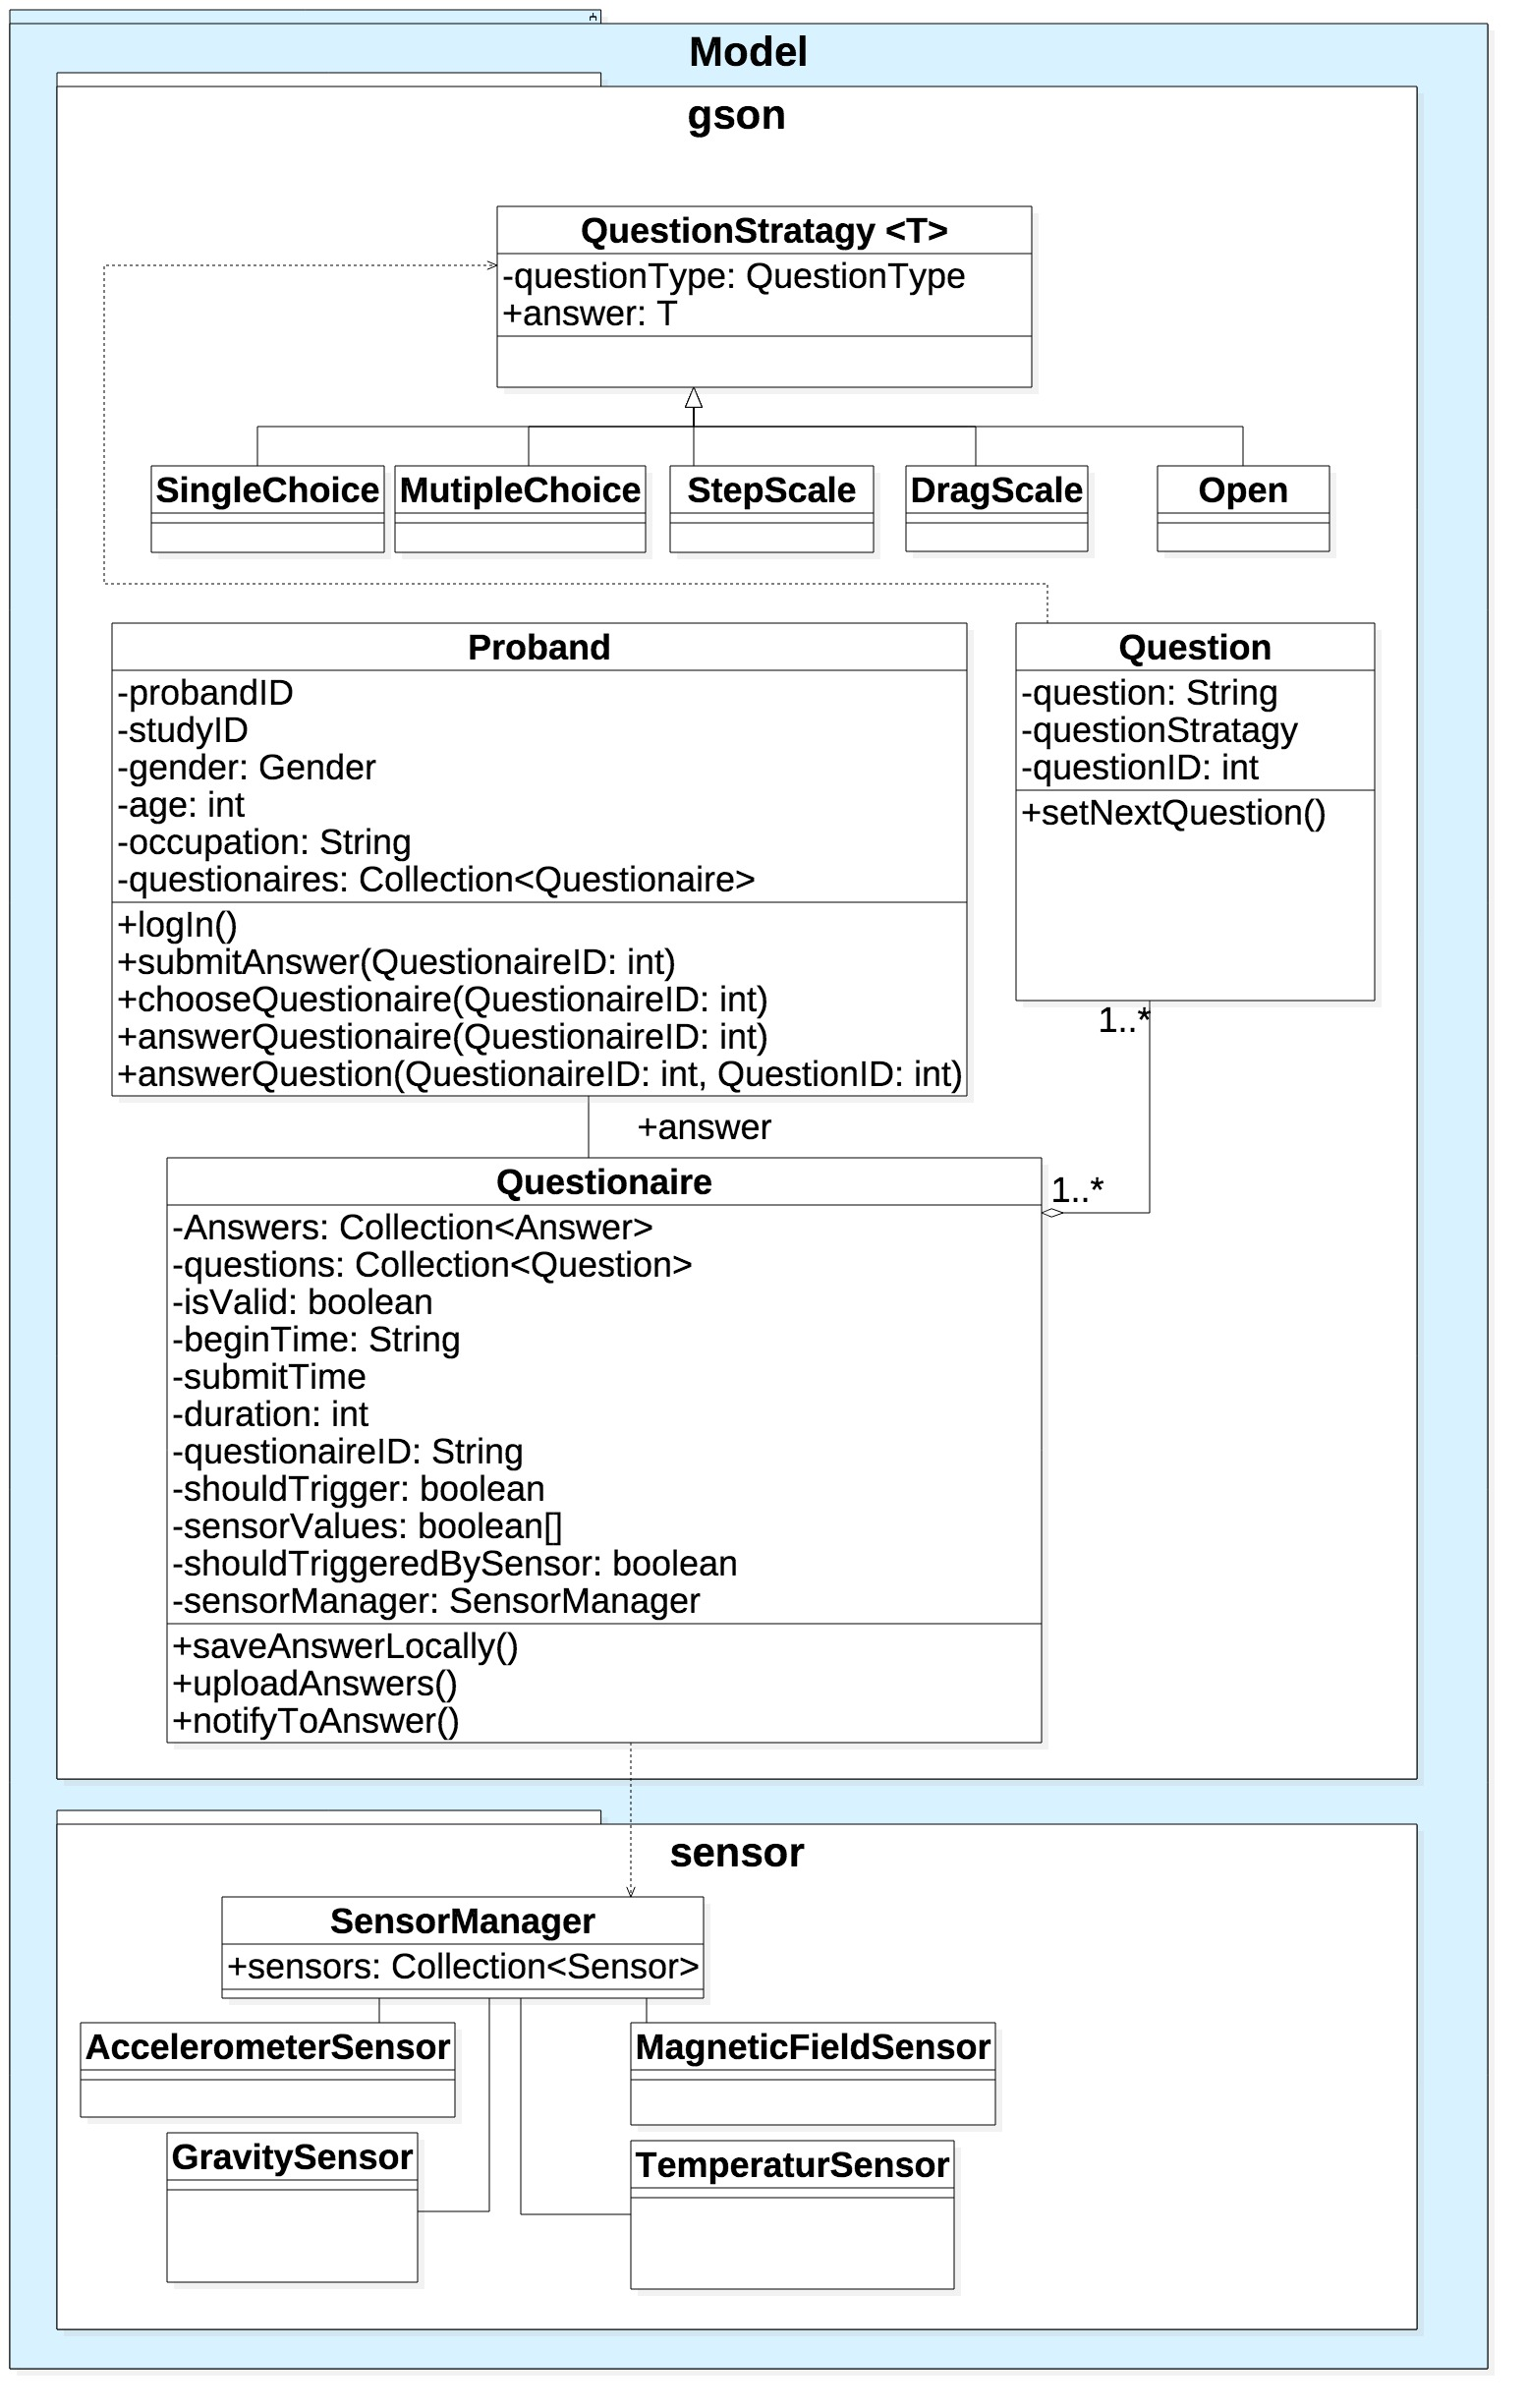
\includegraphics[scale=0.28]{Model.jpg}
                \caption{Model (Modelle)}
            \end{figure}


            \newpage
            \subsection{package \code{gson}}

                \vspace*{1cm}
                \subsubsection{class \code{Proband}}


                    \begin{enumerate}
                        \item Attribute
                            \begin{itemize}
                                \item {\large \code{probandID:String}}\\
                                    die einzige ausgeteilte ID für jeden Proband
                                \item {\large \code{studyID:String}}\\
                                    die ID der Studie
                                \item {\large \code{gender:String}}\\
                                    Geschlecht des Probands
                                \item {\large \code{birthday:String}}\\
                                    Geburtstag des Probands
                                \item {\large \code{occupation:String}}\\
                                    Beruf des Probands
                                \item {\large \code{questionnaires:Collection<Questionnaire>}}\\
                                    alle zu antwortene Fragebögen
                            \end{itemize}

                        \item Methoden
                            \begin{itemize}
                                \item {\large \code{login()}}\\
                                    Nach Aufruf von Methode \code{logIn()} werden folgende Schritte durchgeführt:
                                    \begin{figure}[H]
                                        \centering
                                        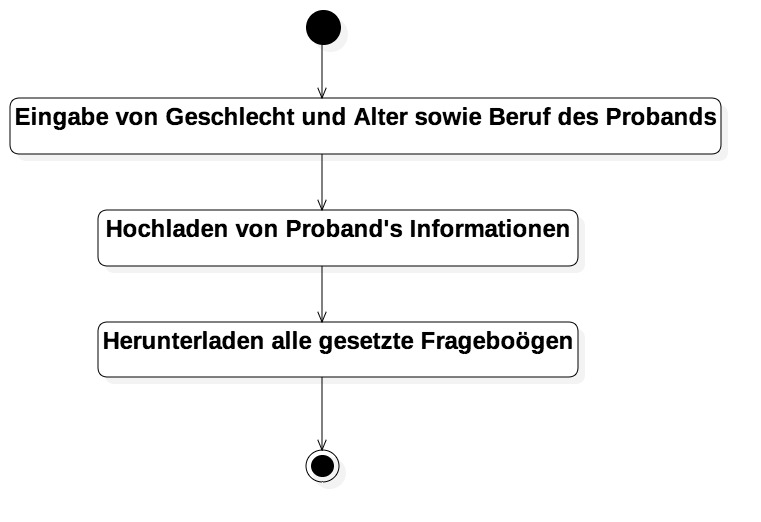
\includegraphics[scale = 0.5]{logIn.jpg}
                                        \caption{\code{logIn()}}
                                    \end{figure}

                                \item {\large \code{submitAnswer(QuestionnaireID:String)}}\\
                                    Nach Klicken von Button ``Submit'' wird diese Methode aufgerufen. Die Antwort von Fragebogen mit \code{QuestionnaireID} wird zuerst lokal gespeichert. Dann versucht unsere Android-App, die Antwort auf den Server hochzuladen.
                                \item {\large \code{chooseQuestionnaire(QuestionnaireID:String):Questionnaire}}\\
                                    Mit \code{QuestionnaireID} kann der Proband dem bestimmten Fragebogen auswählen.
                                \item {\large \code{answerQuestionniare(QuestionnaireID:String)}}\\
                                    Mit \code{QuestionnaireID} kann der Proband dem bestimmten Fragebogen beantworten.
                                \item {\large \code{answerQuestion(QuestionnaireID:String, QuestionID:String)}}\\
                                    Durch Aufruf dieser Methode kann der Proband die bestimmte Frage, deren ID \code{QuestionID} ist, von Questionnaire \code{QuestionnaireID} beantworten.
                                \item {\large setters und getters für alle Attribute}
                            \end{itemize}
                    \end{enumerate}




                \subsubsection{class \code{Questionnaire}}

                    \begin{enumerate}
                        \item Attribute
                            \begin{itemize}
                                \item {\large \code{questions:Collection<Question>}}\\
                                    enthält alle Fragen dieses Fragebogens
                                \item {\large \code{isValid:boolean}}\\
                                    Falls der Proband innerhalb des gültigen Zeitbereich den Fragebogen nicht beantworten, wird den Wert dieser Attribute als ``false'' gesetzt.
                                \item {\large \code{beginTime:String}}\\
                                    Anfangszeitpunkt des Fragebogens
                                \item {\large \code{duration:int}}\\
                                    Dauer des gültigen Zeitbereich
                                \item {\large \code{QuestionnaireID:String}}\\
                                    die einzige ID des Fragebogens
                                \item {\large \code{shouldTrigger:boolean}}\\
                                    ob der Fragebogen ausgelöst werden soll
                                \item {\large \code{sensorValues:boolean[]}}
                                    \begin{itemize}
                                        \item Länge = Anzahl die von Handy angebotenen Sensoren
                                        \item Jeder Sensor entpricht einem Element in dieser Array.
                                        \item Falls der Wert eines Sensors die von Studiensleiter gesetzte Kriterien erfüllt, wird der Wert des entsprechenden Element ``true'' gesetzt. Sonst ``false''.
                                        \item z.B. Die Handy bietet 4 Sensoren an: Accelerometer-Sensor, MagneticFeld-Sensor, Temperature-Sensor und Gravity-Sensor. Die Länge dieser Array ist 4. Das erste Array-Element entspricht Accelerometer-Sensor, die zweite entspricht MagneticFeld-Sensor,usw. Jetzt erfüllen die Werte von Accelerometer-Sensor und MagneticFeld-Sensor die gesetzte Kriterien. Daher sieht \code{sensorValues} so aus: \\
                                        \code{sensorValues = {true, true, false, false}}


                                    \end{itemize}
                                \item {\large \code{shouldTriggeredBySensor:booelan}} \\
                                    Ergebnis der ``and'' Operation mit allen Elemente in \code{sensorValues}\\
                                    z.B. sensorValues = {true, true, false, true}, dann \\
                                    \code{shouldTriggeredBySensor = true \&\& true \&\& false \&\& true = false}
                                \item {\large \code{sensorManager:SensorManager}}\\
                                    Verwaltung von allen Snesoren
                            \end{itemize}
                        \item Methoden
                            \begin{itemize}
                                \item {\large \code{saveAnswerLocally()}}
                                \item {\large \code{uploadAnswer(serverAddress:String)}}\\
                                    Hochladen von Antwort auf den Server mit Adresse \code{serverAddress}
                                \item {\large \code{notifyToAnsewr()}}\\
                                    sendet Handy-Notifikation, um den Proband zu erinnern, die ausgelöste Fragebögen zu beantworten.
                                \item {\large setters und getters für alle Attribute}
                            \end{itemize}
                    \end{enumerate}

                \subsubsection{class \code{Question}}

                    \begin{enumerate}
                        \item Attribute
                            \begin{itemize}
                                \item {\large \code{question:String}}\\
                                    Inhalt der Frage
                                \item {\large \code{questionType: QuestionStrategy}}\\
                                    Art dieser Frage
                                \item {\large \code{questionID: String}}\\
                                    die einzige ID dieser Frage
                                \item {\large \code{nextQuestionID: String}}
                            \end{itemize}
                        \item Methoden
                            \begin{itemize}
                                \item {\large setters und getters für alle Attribute}
                            \end{itemize}
                    \end{enumerate}

                \subsubsection{abstract class \code{QuestionStrategy<T>}} %super abstract class

                    Hier wird Entwurfsmuster Stagtegie (eng: Strategy) eingesetzt, indem \code{QuestionStrategy} als Teil der Aggregation von \code{Question} und gleichzeitig als Oberklasse (eng: super class) von \code{SingleChoice}, \code{MutipleChoice}, \code{StepScale}, \code{DragScale} und \code{TextAnswer} gesetzt wird.
                    \begin{enumerate}
                        \item Attribute
                            \begin{itemize}
                                \item {\large \code{answer:T}}\\
                                    Generische Programmierung (eng:Generic) wird für attribute \code{answer} angewandet, da der Datentyp von Attribute \code{answer} in vershiedener Unterlasse von \code{QuestionStrategy} unterschiedlich sein sollte.
                                % \item \code{}
                                % \item \code{}
                            \end{itemize}
                        \item Methoden
                            \begin{itemize}
                                \item {\large setters und getters für alle Attribute}
                            \end{itemize}
                        \item Unterklasse\\
                            Laut Pflichtenheft gibt es fünf Fragearten. Deswegen gibt es fünf Unterklassen:
                            \begin{itemize}
                                \item {\large class \code{SingleChoice}}
                                \item {\large class \code{MultipleChoice}}
                                \item {\large class \code{StepScale}}
                                \item {\large class \code{DragScale}}
                                \item {\large class \code{TextAnswer}}
                            \end{itemize}
                    \end{enumerate}


            \subsection{package \code{Sensor}}
            \begin{figure}[H]
                \centering
                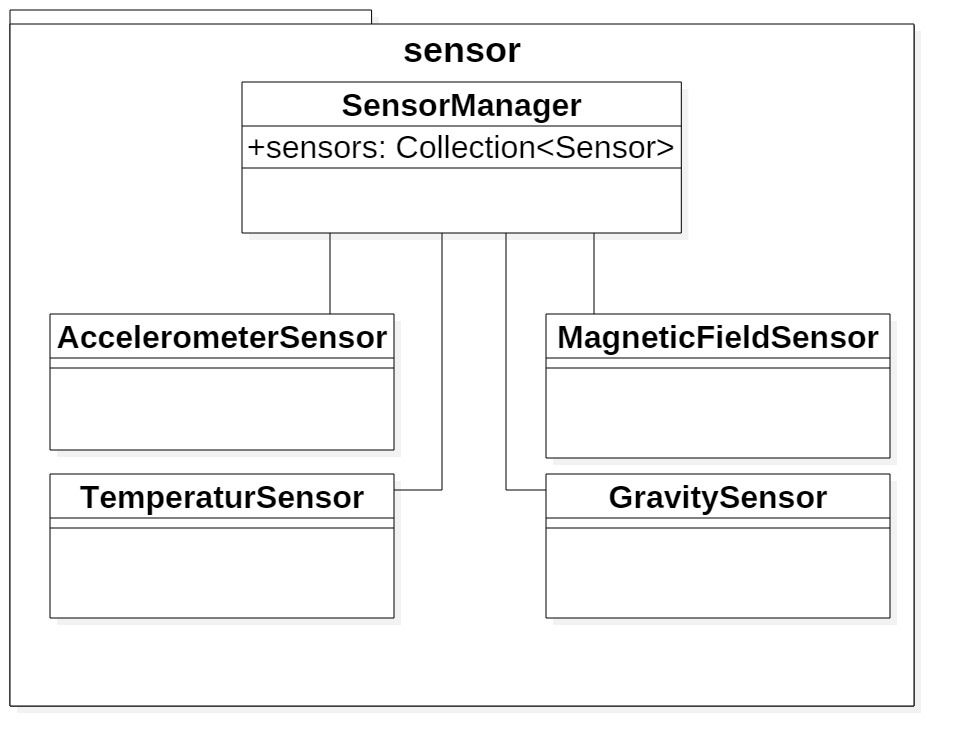
\includegraphics[scale = 0.5]{ClassDiagramAppSensor.jpg}
                \caption{Klassendiagramm für Sensoren in der Android Applikation }
            \end{figure}
                \subsubsection{class \code{SensorManager}}
                Diese Klasse ist einer Manager aller Sensoren, die in diesem Fragebogen bunutzt werden.
                \begin{enumerate}
                  \item Attribute
                    \begin{itemize}
                      \item {\large\code{sensors:Collection<Sensor>}}\\
                      enthält alle Sensoren, die in diesem Fragebogen bunutzt werden.
                    \end{itemize}
                \end{enumerate}
                \subsubsection{class \code{AccelerometerSensor}}
                Diese Klasse handelt sich um den Sensor über Beschleunigung.
                \subsubsection{class \code{GravitySensor}}
                Diese Klasse handelt sich um den Sensor über Gravitation.
                \subsubsection{class \code{MagneticFeldSensor}}
                Diese Klasse handelt sich um den Sensor über Magnetfeld.
                \subsubsection{class \code{TemperatureSensor}}
                Diese Klasse handelt sich um den Sensor über Temperatur

        \newpage
        \section{View}

            Dieser Paket wird automatisch erstellt,  wenn man mit Android Studio ein neues Program erstellt.

            \vspace*{1cm}
            \begin{figure}[H]
                \centering
                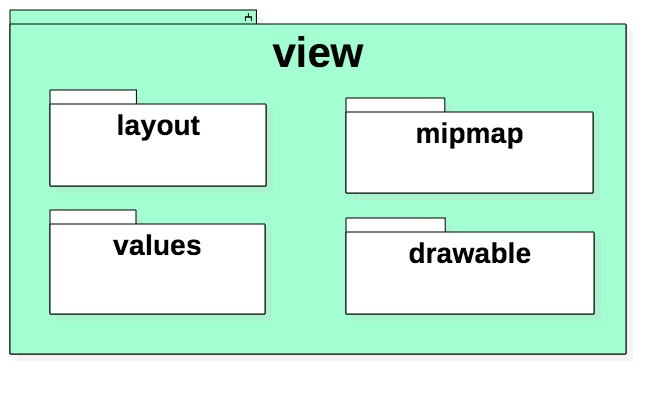
\includegraphics[scale = 0.7]{view.jpg}
                \caption{view (Präsentation)}
            \end{figure}

            \begin{itemize}
                \item {\large layout} \\
                    enthält layout-Datei von \code{Activity} und \code{Fragment}
                \item {\large mipmap} \\
                    enthält die in unsere Android-App verwendete Bilder.
                \item {\large values}\\
                    enthält lokale Ressource für Präsentation (eng: view resource) unserer Android-App.
                \item {\large drawable}\\
                    enthält die in unsere Android-App verwendete Bilder.
            \end{itemize}




        \section{Control}
            Der Teil Control besteht aus zwei Pakete: activity und fragment.

            \vspace*{1cm}
            \begin{figure}[H]
                % \centering
                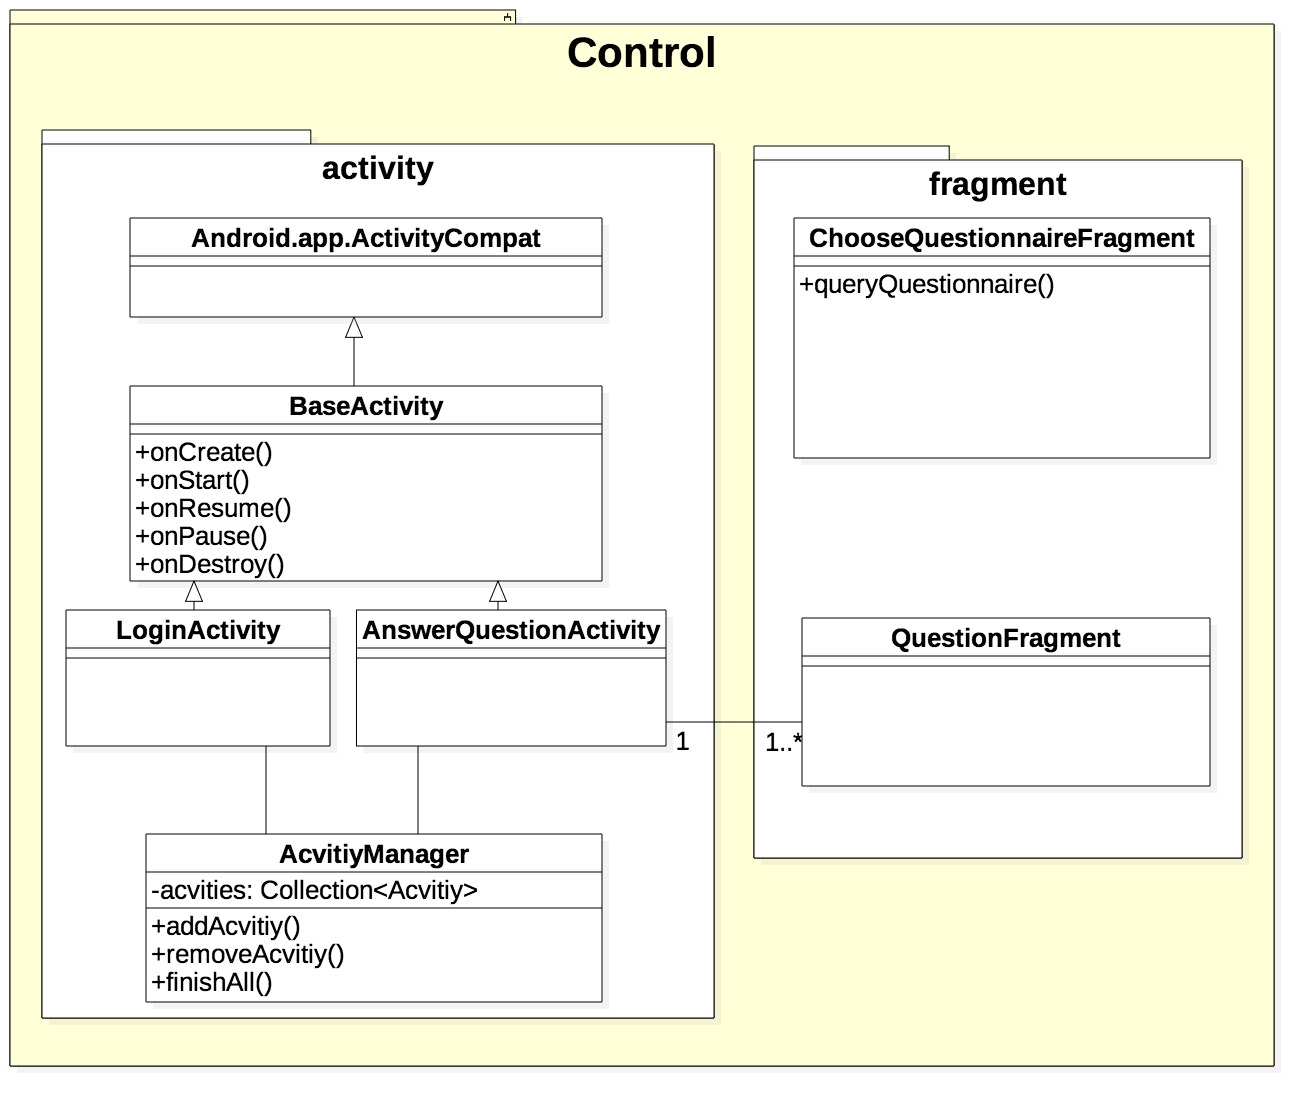
\includegraphics[scale = 0.35]{Control.jpg}
                \caption{Klassendiagramm für Control in der Android Applikation }
            \end{figure}

            \subsection{activity}

                \subsubsection{class \code{ActivityManager}}
                Diese Klasse dient sich als Verwalter aller Aktivitäten. Durch diese Klasse kann ein Benutzer dieser Applikation die auf System laufende Aktivitäten verwalten, z.B. Starten und Beenden einer Aktivität.
                \begin{enumerate}
                \item Attribute
                     \begin{itemize}
                            \item {\large\code{activities: Collection<Activity>}}\\
                            enthält alle Aktivitäten auf System.
                     \end{itemize}
                \item Methoden
                     \begin{itemize}
                                \item {\large addActivity()}\\
                                füget eine Aktivität in den Liste hinzu.
                                \item {\large removeActivity()}\\
                                entfernt eine Aktivität aus den Liste.
                                \item {\large finishAll()}\\
                                schließt alle Aktivitäten in den Liste ab.
                     \end{itemize}
                \end{enumerate}
                \subsubsection{class \code{BaseActivity}}
                \begin{enumerate}
                        \item Attribute
                        \item Methoden
                            \begin{itemize}
                                \item {\large onCreate()}\\
                                Wenn eine Aktivität erste erstellt wird, wird diese Methode angerufen.
                                \item {\large onStart()}\\
                                Wenn eine Aktivität zur Kunde sichtbar wird, wird diese Methode angerufen.
                                \item {\large onResume()}\\
                                Wenn eine Aktivität mit den Kunde  interagiert, wird diese Methode angerufen.
                                \item {\large onPause()}\\
                                Wenn das System eine vorherige Aktivität erstellt, wird diese Methode angerufen.
                                \item {\large onDestroy()}\\
                                Vor die Zerstörung einer Aktivität wird diese Methode angerufen.
                            \end{itemize}
                        \item Unterklassen
                            \begin{itemize}
                                \item {\large class \code{LogInActivity}}\\
                                Anmelden-Aktivität.
                                \item {\large class \code{AnswerQuestionActivity}}\\
                                Fragebogensbeantworten-Aktivität.
                            \end{itemize}

                \end{enumerate}
                % \subsubsection{class \code{LogInActivity}}
                % \begin{enumerate}
                %         \item Attribute
                %         \item Methoden
                % \end{enumerate}
                % \subsubsection{class \code{AnswerQuestionActivity}}
                %  \begin{enumerate}
                %         \item Attribute
                %         \item Methoden
                % \end{enumerate}

            \subsection{fragment}

                \subsubsection{class \code{ChooseQuestionnaireFragment}}
                \begin{enumerate}
                \item Attribute
                \item Methoden
                     \begin{itemize}
                        \item {\large \code{queryQuestionnaire()}}\\
                            zeigt alle zu beantwortene Fragebögen an
                     \end{itemize}
                \end{enumerate}

                \subsubsection{class \code{QuestionFragment}}
                 \begin{enumerate}
                        \item Attribute
                        \item Methoden
                \end{enumerate}


        \newpage
        \section{Hilfpaket}


            \subsection{package \code{service}}

                Die Klassen in diesem Paket handeln sich um die Hintergrunddienste für unsere Android-App. Die Aufgaben, wie z.B., Hochladen von Antworten, sollen im Hintergrund erledigen, falls die Internetverbindung verfügbar ist, während der Nutzer gerade andere Applikation nutzt oder sein Gerät garnicht in der Hand hat.

                \vspace*{0.5cm}
                \begin{figure}[H]
                    \centering
                    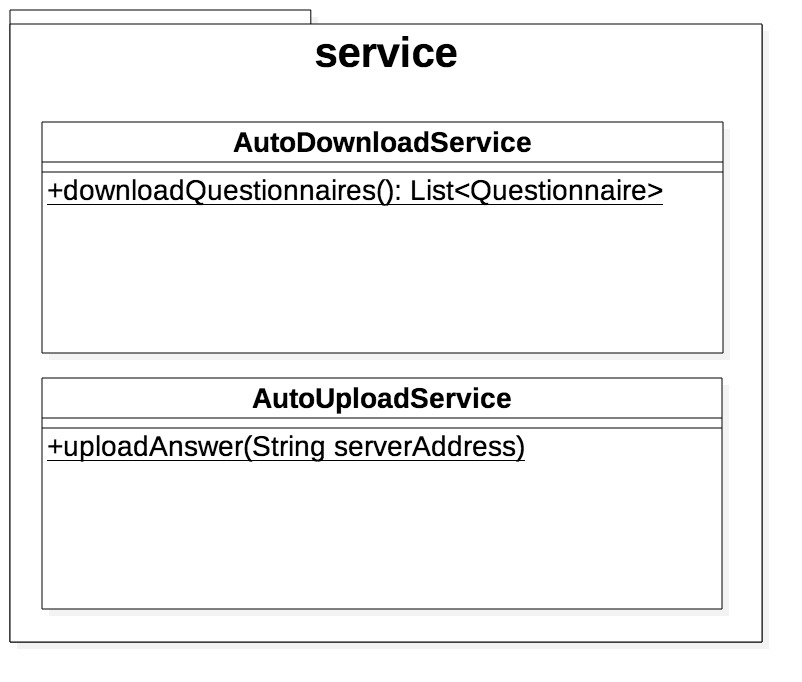
\includegraphics[scale = 0.5]{service.jpg}
                    \caption{package \code{service}}
                \end{figure}

                \subsubsection{AutoDownloadService}
                    \begin{enumerate}
                        \item Attribute
                        \item Methoden
                            \begin{itemize}
                                \item {\large \code{static downloadQuestionnaires(serverAddress:String): List<Questionnaire>}}\\
                                Nach Aufruf von dieser Methode sendet unsere Android-App dem Server Anfrage und lädet alle von studiensleiter gesetzte Fragebögen in Form von JSON-Datei herunter.
                            \end{itemize}
                    \end{enumerate}

                \subsubsection{AutoUploadService}
                    \begin{enumerate}
                        \item Attribute
                        \item Methoden
                            \begin{itemize}
                                \item {\large \code{static uploadAnswer(serverAddress:String)}}\\
                                    lädt die Antwort in Form von JSON-Datei auf den Server hoch
                            \end{itemize}
                    \end{enumerate}

            \newpage
            \subsection{package \code{util}}

                \vspace*{3cm}
                \begin{figure}[H]
                    \centering
                    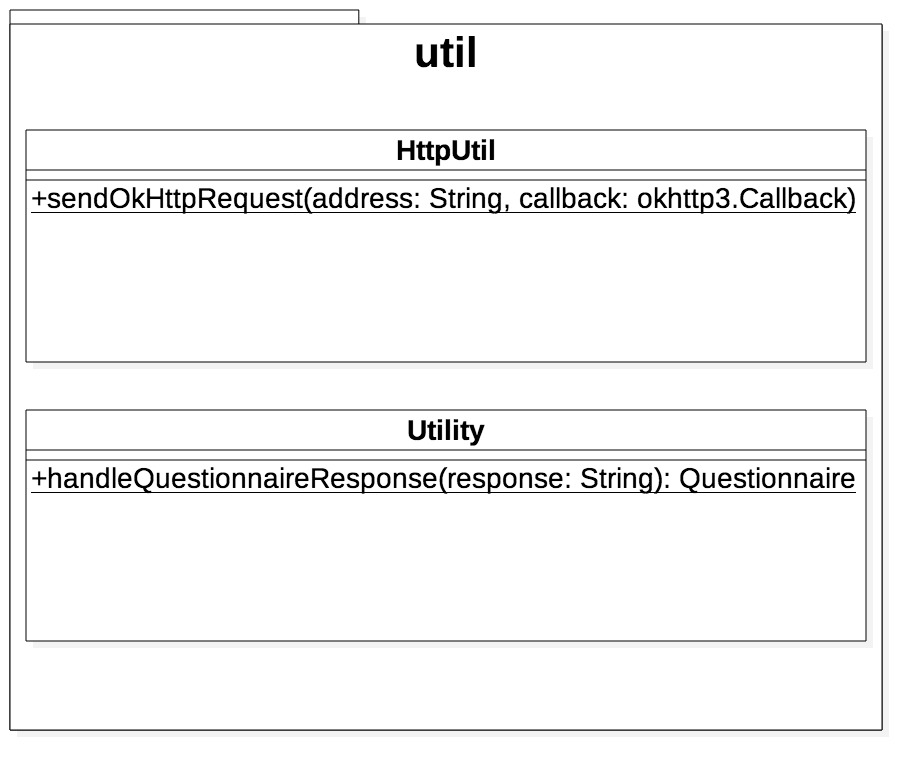
\includegraphics[scale = 0.5]{util.jpg}
                    \caption{package \code{util}}
                \end{figure}

                \subsubsection{class \code{HttpUtil}}

                    Diese Klasse ist zuständig für die Kommunikation zwischen Android-App und Server, indem wir die http-Framework OkHttp\footnote{http://square.github.io/okhttp/} verwenden.

                    \begin{enumerate}
                        \item Attribute
                        \item Methoden
                            \begin{itemize}
                                \item {\large \code{static sendOkHttpRequest(address:String, callback:okhttp3.Callback)}}
                                    sendet dem Server Anfrage mittels OkHttp
                            \end{itemize}
                    \end{enumerate}

                \subsubsection{class \code{Util}}

                    Diese Klasse bietet einige zweckmäßige Funktionen an, z.B. Analysierung der  von Server zurückgegebene Daten.

                    \begin{enumerate}
                        \item Attribute
                        \item Methoden
                            \begin{itemize}
                                \item {\large \code{static handleQuestionnaireResponse(response:String):Questionnaire}}\\
                                Diese Method analysiert die von Server zurückgegebene JSON-Daten und gibt \code{Questionnaire} Objekt zurück.
                            \end{itemize}
                    \end{enumerate}


    \chapter{Interface zwishcen Server und App}
        Die App- und Server-Seiten kommunizieren miteinander per Internet durch das HTTP-Protokoll. Zum Transfer von Daten wird JSON (JavaScript Object Notation) als das Datenformat genutzt.

        \section{Vom Server nach der App}
            \subsection{Anfrage um Proband-Daten}
                Nur die Daten, die vom Studienleiter bestimmt werden, werden an die Probanden gefragt. Eine JSON-Datei als Beispiel:
                
                \lstinputlisting[style=json]{JSON_Examples/require_proband_data_server_to_app.json}

            \subsection{Übertragung der Fragebogen vom Server nach der App}
                Eine JSON-Datei als Beispiel:
                
                \lstinputlisting[style=json]{JSON_Examples/questionnaires_server_to_app.json}


        \newpage
        \section{Von Android-App nach dem Server}

            \subsection{Übertragung der Information des Probands}

                Eine JSON-Datei als Beispiel:

                \lstinputlisting[style=json]{JSON_Examples/Proband_info.json}

% \begin{lstlisting}[style=json]

%     {
%      "probandID" : 123456789,
%      "studyID" : 987654321,
%      "gender" : "male",
%      "birthday": {
%         "year" : 1994,
%         "month" : 1,
%         "day" : 1
%      }
%      "occupation" : "student"
%     }
% \end{lstlisting}


            \subsection{Übertragung der Antwort von Android-App nach dem Server}

                Eine JSON-Datei als Beispiel:

                \lstinputlisting[style=json]{JSON_Examples/Answer.json}

 % \begin{lstlisting}[style=json]

 %    {
 %     "questionnaireID" : 9527,
 %     "duration" : {
 %        "year" : 0,
 %        "month" : 0,
 %        "day" : 20,
 %        "hour" : 12,
 %        "minute" : 0,
 %        "second" : 0
 %     },
 %     "answerSubmitDate" : {
 %        "year" : "2017",
 %        "month" : "1",
 %        "day" : "1",
 %        "hour" : "12",
 %        "minute" : "30",
 %        "second" : "00"
 %     },
 %     "triggerEvent" : [
 %        {
 %            "sensorName" : "AccelerometerSensor", 
 %            "event" : "> 1"
 %        },
 %        {
 %            "sensorName" : "TemperatureSensor", 
 %            "event" : "> 15"
 %        }
 %     ],
 %     "isTriggedBySensor" : true,
 %     "sensors" : [
 %        {
 %         "sensorName" : "AccelerometerSensor",
 %         "value" : 2
 %        },
 %        {
 %         "sensorName" : "TemperatureSensor",
 %         "value" : 20
 %        }
 %     ],
 %     "answers" : [
 %        {
 %         "questionID" : 1,
 %         "type" : "SingleChoice",
 %         "content" : 1
 %        },
 %        {
 %         "questionID" : 2,
 %         "type" : "MutipleChoice",
 %         "content" : [1, 3]
 %        },
 %        {
 %         "questionID" : 3,
 %         "type" : "TextAnswer",
 %         "content" : "Hello world!"
 %        }
 %     ]
 %    }
% \end{lstlisting}



    \glsaddall
    \printglossary

    % Abbildungsverzeichnis
    \listoffigures

\end{document}
